\documentclass[12pt]{article}

\usepackage[T1]{fontenc}
\usepackage{lmodern}
\usepackage[utf8]{inputenc}
\usepackage[american]{babel}

% Page & typography
\usepackage{geometry}
\geometry{margin=1in}
\usepackage{setspace}
\doublespacing
\usepackage{microtype}
\emergencystretch=2em  % loosen linebreaking to avoid overfull boxes
\sloppy                 % last-resort line breaking (safe for drafts)
\usepackage[section]{placeins}

% Line numbers
\usepackage[switch,modulo]{lineno}
\setlength\linenumbersep{10pt} % a bit more space from text
\renewcommand\linenumberfont{\normalfont\small\ttfamily}

% Number sections/subsections
\setcounter{secnumdepth}{3}

% Math, tables, figures
\usepackage{amsmath, amssymb}
\usepackage{graphicx}
\usepackage{booktabs}
\usepackage{threeparttable}
\usepackage{array}
\usepackage{tabularx}
\usepackage{longtable}
\usepackage{caption}
\usepackage{float}
\usepackage{ragged2e}
\usepackage{siunitx}
\sisetup{detect-weight,detect-family,table-number-alignment=center}
\usepackage{makecell}

% Grouping and thousands separator
\sisetup{
  group-separator = {\,},
  group-minimum-digits = 4
}

% - Images: sensible defaults + safe include -
\graphicspath{{figures/}{./}}
\setkeys{Gin}{width=\linewidth,keepaspectratio}
\newcommand{\safeincludegraphics}[2][]{\includegraphics[#1]{#2}}

% Colors
\usepackage{xcolor}

% Captions: avoid wide lines
\captionsetup{
  font=small,
  justification=raggedright,
  singlelinecheck=false
}

% Tabularx helpers
\newcolumntype{Y}{>{\RaggedRight\arraybackslash}X}
\renewcommand{\arraystretch}{1.15}

% Authors & affiliations
\usepackage{authblk}
\makeatletter
\newcommand{\samethanks}[1][\value{footnote}]{\footnotemark[#1]}
\makeatother

% Bibliography (APA, author-year)
\usepackage{csquotes}
\usepackage[style=apa, backend=biber, maxcitenames=2, uniquelist=false]{biblatex}
\DeclareLanguageMapping{american}{american-apa}

\addbibresource{references.bib} % ensure this file exists

% Links (break long URLs/DOIs safely)
\usepackage{xurl} % smarter URL breaking
\usepackage[unicode,breaklinks=true]{hyperref}
\hypersetup{
  colorlinks=true,
  urlcolor=blue,
  linkcolor=black,
  citecolor=black
}

% (Optional) Tighter, compressed PDF output
\pdfminorversion=7
\pdfcompresslevel=9
\pdfobjcompresslevel=3

% TikZ for architecture diagram
\usepackage{tikz}
\usetikzlibrary{positioning, fit, backgrounds, arrows.meta}

% Metadata
\title{A Multi-Agent Orchestration Framework for Venture Capital Due Diligence}
\author[2]{Grigorios Alexandrou}
\author[2]{Katerina Pramatari\thanks{Supervising professor.}}
\affil[2]{Department of Management Science and Technology,
Athens University of Economics and Business (AUEB), Athens, Greece}
\date{\today}

\begin{document}
\maketitle
\linenumbers

\begin{abstract}
  We present a fully automated multi-agent framework for corporate due diligence and market
  analysis in venture capital. The system runs on an event-driven orchestration architecture,
  combining Large Language Models (LLMs) with real-time web retrieval to synthesize unstructured
  data into investment intelligence. A core component reverse-engineers the frontend-to-backend
  communication of the Greek Business Registry ($\Gamma$.E.MH.), querying dynamic endpoints and
  applying Optical Character Recognition (OCR) to extract data from official financial filings
  and corporate records. When registry data is absent, a structural fallback queries alternative
  financial databases rather than generating unverified figures. Together, these components show
  that modular agentic workflows can substantially reduce analyst time in due diligence while
  preserving data provenance.
\end{abstract}

\textbf{Keywords:} AI agents; Workflow Automation; Due Diligence; Venture Capital; Financial Intelligence; Large Language Models; Hallucination Mitigation

\section{Introduction}
\label{sec:intro}

Evaluating prospective investments and monitoring portfolio companies demands synthesis of
fragmented information across incompatible sources: unstructured web data, real-time news,
competitive analyses, and official financial registries that are often locked behind
administrative access controls. Manual desk research, the standard approach, introduces human
error, cognitive bias, and delays that compound across a portfolio
\parencite{gompers2016private, kahneman2011thinking}.

LLMs offer new capabilities for natural language understanding and data synthesis
\parencite{bommasani2021opportunities}, but deploying them for financial due diligence has three
structural problems. Training data cut-offs leave models blind to current market signals. Models
generate plausible but factually wrong information, a failure mode investment decisions cannot
tolerate \parencite{ji2023survey}. And LLMs cannot independently query external databases, call
APIs, or parse scanned financial PDFs \parencite{wu2023autogen}.

We address these problems with a fully automated, multi-agent orchestration pipeline. Rather than
a single LLM prompt, the system decomposes due diligence into specialized sub-tasks handled by
distinct AI agents \parencite{xi2023rise}. Real-time search APIs supply current market
intelligence; custom extraction modules programmatically retrieve and parse official financial
filings from the Greek Business Registry ($\Gamma$.E.MH.).

This paper makes three contributions: (1) a modular, multi-agent architecture that automates
end-to-end corporate research; (2) a programmatic extraction pipeline that queries hidden
registry endpoints, retrieves PDF documents, and applies OCR to structure financial data; and
(3) a structural fallback mechanism that switches to open-source intelligence when official
registry data is unavailable, replacing unverifiable LLM outputs with explicit data gaps
\parencite{gao2023retrieval}.

\section{Background and Related Work}
\label{sec:background}

The field has moved from single-prompt LLM interactions toward Agentic Workflows, where multiple
LLM-powered entities each carry distinct roles, system prompts, and tool-use capabilities
\parencite{xi2023rise}. Chaining agents lets each one hand its verified output to the next,
building reasoning chains too complex for a single model call. Multi-step analytical problems,
which require precision and iterative correction, are the natural fit for these architectures
\parencite{wu2023autogen}.

Applying these systems to finance is natural: general LLMs struggle with specialized vocabulary
and numerical precision \parencite{yang2023fingpt}. Instruction tuning combined with real-time
data feeds yields more precise risk assessment and market sentiment analysis
\parencite{wu2023bloomberggpt}. Frameworks such as MARAG-Fin and QuantAgents go further,
distributing analytical tasks across specialized agents to improve accuracy and reduce
hallucinations in volatile markets \parencite{maragfin2025, li2025quantagents}. Investment
analysis has become a productive testbed for task-specific agentic pipelines.

Dynamic information retrieval addresses the static knowledge problem: grounding model outputs in
real-time search results and external data streams lets systems sidestep training cut-offs
entirely \parencite{lewis2020retrieval}. For corporate intelligence, Open-Source Intelligence
(OSINT) provides current market sizes, funding rounds, and competitor movements.
Retrieval-Augmented Generation makes that intelligence verifiable by linking outputs to primary
sources \parencite{gao2023retrieval}.

Automated OCR and document processing extend this reach into non-digitized corporate records.
Layout-aware parsers can handle balance sheets and income statements without the structural loss
common to older engines \parencite{paruchuri2025marker}. Combined with real-time web retrieval,
these tools give workflows a path from fragmented market signals to formal regulatory filings in
a single pipeline \parencite{bommasani2021opportunities}.

\section{System Architecture}
\label{sec:architecture}

The system runs on an event-driven automation platform \parencite{n8n2024}, structured as a
Directed Acyclic Graph (DAG) of processing nodes. A custom HTML form acts as the entry point
for investment teams: analysts select a target portfolio company and trigger the full research
workflow with a single click, with the low-code backend hidden from view.

\begin{figure}[htbp]
  \centering
  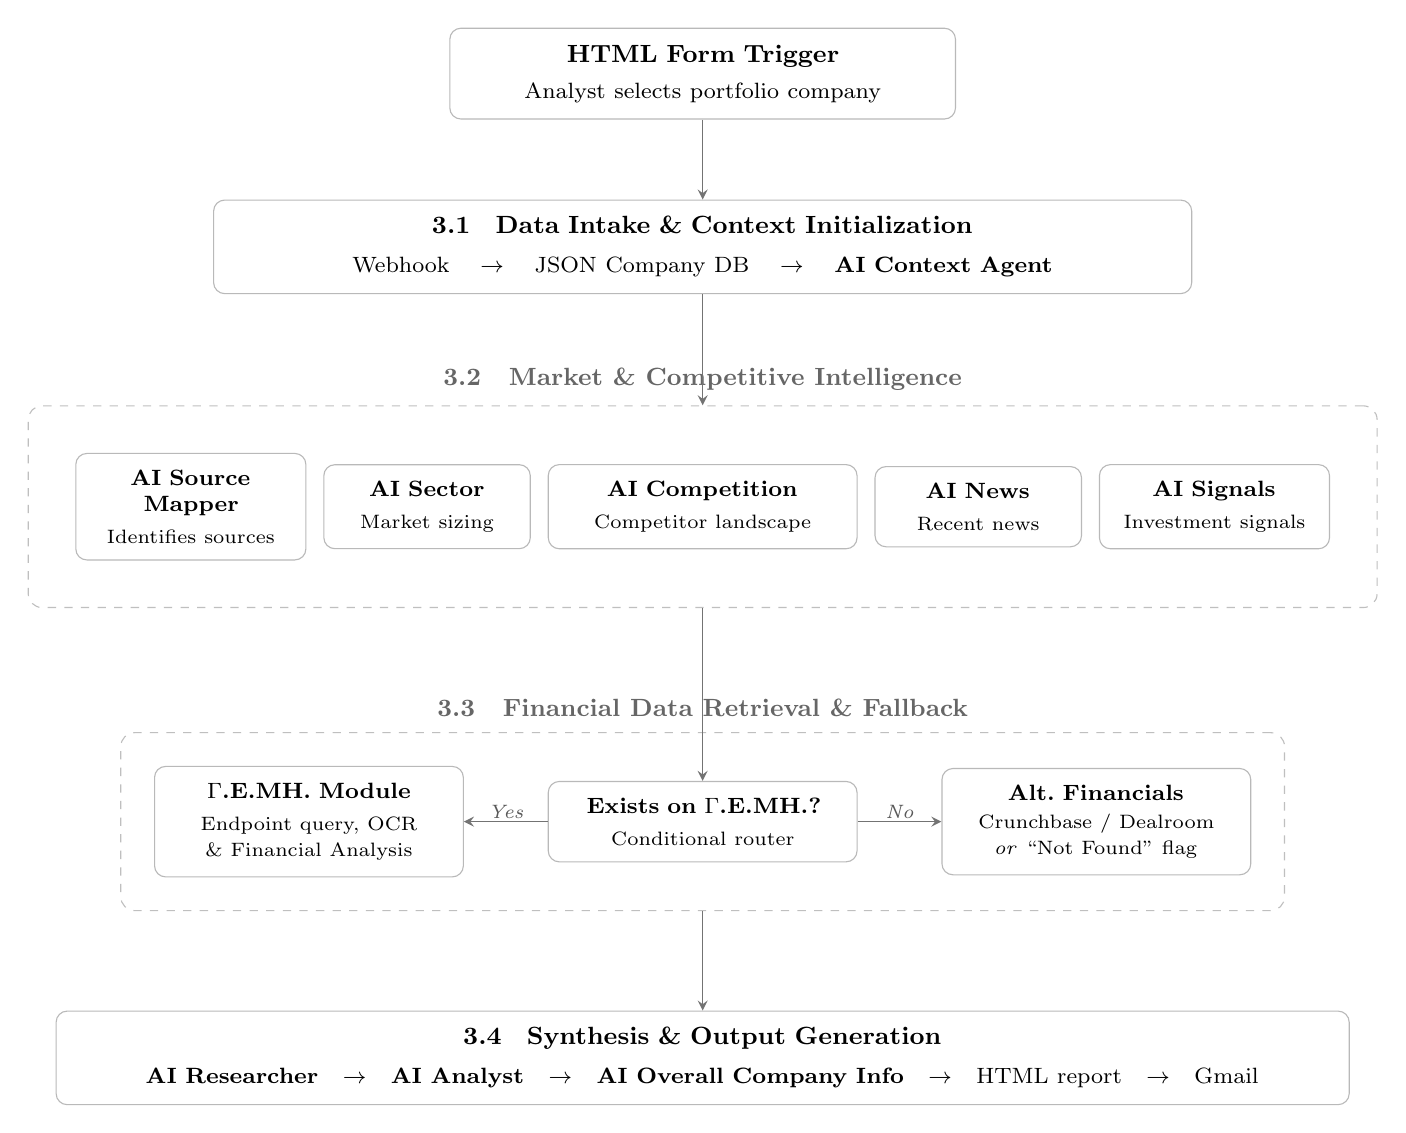
\begin{tikzpicture}[
      arr/.style={->, >=stealth, semithick, black!55},
      lbl/.style={draw=none, fill=none, font=\scriptsize\itshape,
          black!65, inner sep=1pt},
      boxnode/.style={rectangle, rounded corners=4pt, draw=gray!55,
          fill=white, align=center, font=\small, inner sep=6pt},
    ]

    %% ── TRIGGER  (y=0) ──────────────────────────────────────────────────────
    \node[boxnode, text width=6cm] at (0, 0) (trigger)
    {\textbf{HTML Form Trigger}\\[2pt]
    {\footnotesize Analyst selects portfolio company}};

    %% ── 3.1  (y=-2.2) ───────────────────────────────────────────────────────
    \node[boxnode, text width=12cm] at (0, -2.2) (intake)
    {\textbf{3.1 \; Data Intake \& Context Initialization}\\[3pt]
    {\footnotesize Webhook $\;\rightarrow\;$ JSON Company DB
    $\;\rightarrow\;$ \textbf{AI Context Agent}}};

    %% ── 3.2 agents  (y=-5.5, leaving room for group label at y≈-4.0) ───────
    \node[boxnode, text width=2.5cm, font=\footnotesize] at (-6.5, -5.5) (mapper)
    {\textbf{AI Source Mapper}\\[2pt]{\scriptsize Identifies sources}};
    \node[boxnode, text width=2.2cm, font=\footnotesize] at (-3.5, -5.5) (sector)
    {\textbf{AI Sector}\\[2pt]{\scriptsize Market sizing}};
    \node[boxnode, text width=3.5cm, font=\footnotesize] at ( 0.0, -5.5) (competition)
    {\textbf{AI Competition}\\[2pt]{\scriptsize Competitor landscape}};
    \node[boxnode, text width=2.2cm, font=\footnotesize] at ( 3.5, -5.5) (news)
    {\textbf{AI News}\\[2pt]{\scriptsize Recent news}};
    \node[boxnode, text width=2.5cm, font=\footnotesize] at ( 6.5, -5.5) (signals)
    {\textbf{AI Signals}\\[2pt]{\scriptsize Investment signals}};

    \begin{scope}[on background layer]
      \node[draw=gray!50, fill=white, dashed, rounded corners=5pt,
        inner sep=17pt,
        fit=(mapper)(sector)(competition)(news)(signals),
        label={[draw=none, fill=none, font=\small\bfseries, black!60,
                anchor=south, yshift=2pt]above:%
            3.2 \; Market \& Competitive Intelligence
          }]
      (group32){};
    \end{scope}

    %% ── 3.3 nodes  (y=-9.5, leaving room for group label at y≈-7.8) ────────
    \node[boxnode, text width=3.5cm, font=\footnotesize] at (-5.0, -9.5) (gemh)
    {\textbf{$\Gamma$.E.MH.\ Module}\\[2pt]
    {\scriptsize Endpoint query, OCR \& Financial Analysis}};
    \node[boxnode, text width=3.5cm, font=\footnotesize] at ( 0.0,  -9.5) (router)
    {\textbf{Exists on $\Gamma$.E.MH.?}\\[2pt]
    {\scriptsize Conditional router}};
    \node[boxnode, text width=3.5cm, font=\footnotesize] at ( 5.0, -9.5) (altfin)
    {\textbf{Alt.\ Financials}\\[2pt]
    {\scriptsize Crunchbase / Dealroom\\
    \textit{or} ``Not Found'' flag}};

    \begin{scope}[on background layer]
      \node[draw=gray!50, fill=white, dashed, rounded corners=5pt,
        inner sep=12pt,
        fit=(gemh)(router)(altfin),
        label={[draw=none, fill=none, font=\small\bfseries, black!60,
                anchor=south, yshift=2pt]above:%
            3.3 \; Financial Data Retrieval \& Fallback}]
      (group33){};
    \end{scope}

    %% ── 3.4 ─────────────────────────────────────────────────────────────────
    \node[boxnode, text width=16cm] at (0, -12.5) (synthesis)
    {\textbf{3.4 \; Synthesis \& Output Generation}\\[3pt]
    {\footnotesize \textbf{AI Researcher} $\;\rightarrow\;$
    \textbf{AI Analyst} $\;\rightarrow\;$
    \textbf{AI Overall Company Info} $\;\rightarrow\;$
    HTML report $\;\rightarrow\;$ Gmail}};

    %% ── ARROWS ──────────────────────────────────────────────────────────────
    \draw[arr] (trigger)       -- (intake);
    \draw[arr] (intake)        -- (group32.north);
    \draw[arr] (group32.south) -- (router.north);
    \draw[arr] (router.west)   -- node[lbl, above]{Yes} (gemh.east);
    \draw[arr] (router.east)   -- node[lbl, above]{No}  (altfin.west);
    \draw[arr] (group33.south) -- (synthesis.north);

  \end{tikzpicture}
  \caption{High-level overview of the event-driven multi-agent orchestration
    architecture, structured according to the four pipeline stages described
    in Sections~\ref{sec:architecture}--\ref{sec:output}.}
  \label{fig:architecture}
\end{figure}


\subsection{Data Intake and Context Initialization}
On submission, a Webhook node captures the payload. A transformation node maps the selected
company to a pre-scraped JSON database of baseline attributes: founders, sector, initial
investment year, headquarters, and registration numbers. The \textbf{AI Context Agent} takes
this input and produces a compact company profile that anchors all downstream research nodes.

\subsection{Market and Competitive Intelligence Modules}
Five specialized agents query the Perplexity Sonar Deep Research API
\parencite{perplexity2024sonar} for real-time market intelligence. The \textbf{AI Source Mapper}
runs first, identifying the most reliable sector-specific portals, databases, and news
aggregators for the target company. The \textbf{AI Sector} and \textbf{AI Competition} agents
run in parallel against those sources, extracting market sizing, macro-environmental trends, and
a competitive landscape that categorizes competitors as direct, adjacent, or niche innovators.
Once both complete, the \textbf{AI News} and \textbf{AI Signals} agents scan for recent
strategic developments (partnerships, product launches) and extract quantifiable investment
signals.

\subsection{Financial Data Retrieval and Fallback Mechanisms}
\label{sec:financials}

The most complex component interfaces with the Greek Business Registry ($\Gamma$.E.MH.).
Although the registry provides an official API, obtaining authenticated credentials carries
administrative overhead. Instead, the framework reverse-engineers the platform's
frontend-to-backend communication, a method validated by prior open-source work targeting the
same registry \parencite{drakakis2025govdoc}.

Registry data and corporate announcements are served as PDF documents, loaded by the public
portal from specific backend endpoints. A conditional router (Switch/If nodes) checks for a
valid registry number (arGEMI). When one exists, an HTTP Request node mimics the browser's
behavior, querying those endpoints directly to retrieve the JSON payload of required document
IDs.

Document IDs are sorted into two streams: \textbf{Corporate Modifications (Announcements)},
covering board changes, capital increases, and statutory modifications; and \textbf{Financial
Statements}, comprising official balance sheets, income statements, and auditor reports.

The pipeline fetches raw PDF files (prioritizing the most recent fiscal years) and runs them
through a layout-aware text extractor \parencite{paruchuri2025marker}. Two summarization models,
\textbf{AI FinSummary} and \textbf{AI ModSummary}, then distill the extracted text into
standardized financial metrics (Assets, Liabilities, Revenue, EBIT) with source citations
preserved.

Preventing fabricated financial data is the system's hardest constraint. When the initial
routing finds no $\Gamma$.E.MH. number (typically companies incorporated abroad), the pipeline
skips the registry branch and activates the \textbf{Alternative Financials} agent, which queries
Crunchbase, Dealroom, and similar open-source databases. If those sources return nothing, the
agent writes a ``Not Found'' flag directly into the report, making data gaps explicit rather
than filling them with generated figures.

\subsection{Synthesis and Output Generation}
\label{sec:output}

Three synthesis agents combine the intelligence streams. The \textbf{AI Researcher} aggregates
sector, competition, news, signals, and financial data into a strategic research note that
surfaces recent developments and blind spots. The \textbf{AI Analyst} takes that note and
produces an Executive Summary, assigns attractiveness scores across market timing and product
differentiation, and drafts 30-to-180-day recommendations for both the fund and the startup.
The \textbf{AI Overall Company Info} agent generates a public-facing summary founders can use
to understand their external market footprint.

A formatting node converts the JSON outputs into a styled HTML report and dispatches it to the
requesting analyst through a Gmail API integration.

\section{Data and Workflow Availability}
\label{sec:data}
All system artifacts are publicly available in a dedicated repository
\parencite{alexandrou2026due}: the n8n JSON workflow file, project documentation, and an
explanatory video walk-through. Consult the repository documentation for the required
environment variables and node configurations before attempting replication.

\section{Conclusions and Future Work}
\label{sec:conclusion}

Multi-agent orchestration can automate corporate due diligence at a level of reliability
previously requiring human analysts. By combining dynamic web retrieval, reverse-engineered
endpoint querying, and OCR-based document processing, the n8n pipeline connects unstructured
market signals to official financial compliance data in a single automated pass. Structural
fallback mechanisms prevent the system from generating unverified financial figures, replacing
hallucinated outputs with explicit data gaps.

Three directions extend this work. First, integrating the pipeline with the fund's internal
portfolio database would let each report draw on proprietary deal-level data, historical
performance metrics, and analyst notes specific to each startup, making the output contextual
rather than general. Second, adding international registries such as UK Companies House
\parencite{companieshouse2025} and equivalent European authorities would extend coverage to
companies incorporated outside Greece. Third, replacing the third-party PDF extraction API with
a self-hosted open-source alternative would cut operational costs and remove the external
dependency without degrading extraction quality.


\printbibliography

\end{document}
